\chapter{FHTBoost: A multidimensional component-wise gradient boosting algorithm for survival data}
\label{ch:FHTboost}
In this chapter, we propose a component-wise boosting algorithm for fitting the inverse Gaussian first hitting time (FHT) model to survival data.
The algorithm is designed to be especially fit for use with both clinical and genomic data.
We work with survival data sets with $N$ observations,
\begin{equation*}
    D=(\x_i,\z_i,t_i,d_i)_{i=1}^N.
\end{equation*}
Here $t_i$ is a possibly right-censored event time, $d_i$ is an indicator variable which is 1 if $t_i$ is an actually observed event time, and 0 if it is right-censored.
For simplicity later, we denote the response data
\begin{equation*}
    y_i=(t_i,d_i).
\end{equation*}
Further, we have covariate vectors $\x_i$ and $\z_i$, which will be related to the inverse Gaussian parameters $y_0$ and $\mu$, respectively.
$\x_i$ is defined as
\begin{equation}
    \x_i=(x_{i,1},x_{i,2},\ldots,x_{i,p_1}).
\end{equation}
$\z_i$ is defined as
\begin{equation}
    \z_i=(\z_{i,1},\z_{i,2},\ldots,\z_{i,p_2}).
\end{equation}
Typically the number of dimensions $p_1$ of $\x_i$ is high (in particular, $p_1$ is much larger than $n$, $p_1 >> n$), and the number of dimensions $p_2$ of $\z_i$ is relatively small, and in particular, $p_2 < N$.
However, the dimensions $p_1$ and $p_2$ can be any size.
There are theoretical arguments for this particular combination of the high and low-dimensional vectors and parameters, which we have discussed earlier in subsection \ref{subsec:FHT-combine}.

\section{Setting}
\subsection{Additive predictors etc}
The first-hitting-time model with Wiener processes, as shown, leads to inverse Gaussian lifetimes.
The probability distribution function (pdf) for this distribution is given in \eqref{eq:ig-pdf}, and its cumulative distribution function is given in \eqref{eq:ig-cdf}.
The log likelihood is given in \eqref{eq:loglik}.
We repeat it here.
It depends on $y_0$ and $\mu$, and $\sigma$ is in practice set to 1 to avoid overparameterization (see subsection \ref{subsec:overdetermined}).
\begin{align*}
\begin{split}
    l(y_0,\mu|y_i)=\sum_{i=1}^n&d_i\p*{\ln y_0-\frac{1}{2}\ln\p*{2\pi\ti^3}-\frac{\p*{\mu\ti+y_0}^2}{2\ti}} \\
    &+
    (1-d_i)\ln\p*{\Phi\p*{\frac{\mu\ti+y_0}{\sqrt{\ti}}}-\exp\p*{-2y_0\mu}\Phi\p*{\frac{\mu\ti-y_0}{\sqrt{\ti}}}}.
\end{split}
\end{align*}
We wish to use a similar setup as the GAMLSS.
We will therefore model the parameters through additive predictors $\boldeta$, consisting of components $\eta_1$ and $\eta_2$, which we relate by link functions.
We denote the $K=2$ distribution parameters as
\begin{equation}
    \btheta=(\theta_1,\theta_2)^T=(y_0,\mu)^T.
\end{equation}
We relate the parameters to the additive predictors to use the usual link functions
\begin{equation}
    g_1(y_0)=\ln(y_0)
\end{equation}
and
\begin{equation}
    g_2(\mu)=\mu,
\end{equation}
and we further relate the additive predictors to covariates.
The additive predictors for an individual $i$ are defined as
\begin{equation}
    \eta_{1,i}\coloneqq \ln(y_{0,i})=\bbeta^T \x_i=\beta_{0}+\sum_{j=1}^{p_1}x_{j,i}\beta_j
\end{equation}
and
\begin{equation}
    \eta_{2,i}\coloneqq \mu_{i}=\bgamma^T \z_i=\gamma_{0}+\sum_{j=1}^{p_2}z_{j,i}\gamma_j,
\end{equation}
and we denote both as $\boldeta_i=\left(\eta_{1,i},\eta_{2,i}\right)$.

We are going to build up these additive predictors by means of gradient boosting.
Each 

\subsection{Loss function}
Since we have a probability distribution, we should use the negative of the corresponding log likelihood as our loss function.
For an observation numbered $i$ and with parameter vector
\begin{equation*}
    \btheta(\x_i,\z_i)=\left(y_0(\x_i),\mu(\z_i)\right),
\end{equation*}
the loss function is
\begin{equation*}
    \rho(y_i,\hat{\btheta}(\x_i,\z_i))=-l(\hat{y}_{0,i},\hat{\mu}_i|y_i).
\end{equation*}

Given an estimated additive predictor $\hat{\boldeta}$, we calculate the corresponding estimated distribution parameters by transforming the additive predictors via the inverse of their link functions.
Thus,
\begin{equation}
    y_0=\theta_1=g_1^{-1}(\eta_1)=\exp(\eta_1),
\end{equation}
and
\begin{equation}
    \mu=\theta_2=g_2^{-2}(\eta_2)=\eta_2.
\end{equation}
This means that as a function of the additive predictors, the loss function is
\begin{equation*}
    \rho(y,\boldeta)=-l(\exp(\eta_1), \eta_2).
\end{equation*}
To use the gradient boosting algorithm, we need to compute the negative gradient of the loss function, i.e., the negative of the derivative. 
The negative partial derivative of the loss function is equal to the (positive) derivative of the (positive) log-likelihood function, with regard to each parameter.
These are
\begin{equation}
    -\frac{\partial}{\partial\eta_1}\rho(y_i,\btheta)=\frac{\partial}{\partial\eta_1}l(\exp(\eta_1), \eta_2)=f_1
\end{equation}
and
\begin{equation}
    -\frac{\partial}{\partial\eta_2}\rho(y_i,\btheta)=\frac{\partial}{\partial\eta_1}l(\exp(\eta_1), \eta_2)=f_2.
\end{equation}
See Appendix for the full details.

We can now apply the component-wise multidimensional boosting algorithm shown in the previous chapter.
We choose to use the noncyclical variant as this leads to equally good results and is less computationally intensive to tune, due to a one-dimensinal stopping parameter search, as stated in \citet{schmid}.
\todo[inline]{More details here!}

\section{Initialization via maximum likelihood estimate}
To ensure proper estimation of $\eta_1$ and $\eta_2$, we need to compute the intercepts $\beta_{0}$ and $\gamma_{0}$, which capture the general, average effect of the covariates.
If analytical relationships or formulas exist, such as taking the average of a Gaussian distributed variable in an ordinary regression setting, their computation would be straightforward.
In lieu of such known formulas, a reasonable method to use is to perform numerical maximization of the log-likelihood, treating the log likelihood as a function of
\begin{equation*}
    \bbeta_0=\left(\beta_{0},\gamma_{0}\right)
\end{equation*}
only.
Hence the offsets are estimated to be
\begin{equation*}
    \hat{\bbeta}=\argmin_{\bbeta}\err\left(\bbeta\right).
\end{equation*}
To do this in practice, we use the routine called \verb|nlm|, which belongs to the base package of \verb|R|.
\todo[inline]{Find citation for R programming language!}

%\begin{algorithm}
\section{The FHTBoost algorithm}
\label{algo:fhtboost}
\begin{enumerate}
    \item
        Given a survival data set $D=(\x_i, \z_i, t_i,d_i)_{i=1}^N$, where for each observation $i$, $\x_i$ is a vector of clinical measurements,
        $\z_i$ a vector of gene expressions, $t_i$ is the possibly right-censored survival time, and $d_i$ is the censoring indicator. 
        (If $\X$ and/or $\Z$ are not normalized, do this.)
        We wish to estimate the $\hat{\boldeta}$ that minimizes the training error in $\mstop$ number of iterations,
        \begin{equation*}
            \hat{\boldeta}=\argmin_{\boldeta}\err(\boldeta)
        \end{equation*}
    \item
        Set iteration counter $m$ to $0$.
        Initialize additive predictors $\hat{\boldeta}=(\hat{\eta}_1, \hat{\eta}_2)$ to $\hat{\bbeta}_0=\left(\hat{\beta}_{0},\hat{\gamma}_{0}\right)$, by finding maximum likelihood constants through numerical maximization,
        \begin{equation*}
            \hat{\bbeta}=\argmin_{\bbeta}\err\left(\bbeta\right).
        \end{equation*}
    \item
    \label{algostep:FHT-base-learner}
        Specify linear least squares base learners:
        \begin{align*}
            \mathcal{H}_1&=\{h_{1,j}\}_{j=1}^{p_1}=\{x_j\beta_j\}_{j=1}^{p_1}, \\
            \mathcal{H}_2&=\{h_{2,j}\}_{j=1}^{p_1}=\{z_j\gamma_j\}_{j=1}^{p_2}
        \end{align*}
    \item
    \label{algostep:FHT-init}
        Increase $m$ by 1.
    \item
        Compute the negative partial derivative $-\frac{\partial\rho}{\partial \hat{\eta}_1}$
        and evaluate at $\hat{\boldeta}^{[m-1]}(\x_i,\,\z_i),i=1,\ldots,N$, yielding negative gradient vector
        \begin{equation}
            \u^{[m-1]}_1=\left(-\frac{\partial}{\partial \hat{\eta}_1}\rho(y_i, \hat{\boldeta}^{[m-1]}(\x_i,\z_i))\right)_{i=1}^N
        \end{equation}
    \item
        Fit the negative gradient vector to each of the $p_1$ components of $\X$ (i.e. to each base learner) separately, using the base learners specified in step \ref{algostep:FHT-base-learner}, so i.e., fitting
        \begin{equation*}
            \hat{\beta}^{[m]}_{j}=\left(\x_j^T\x_j\right)^{-1}\x_j^T\u^{[m-1]}_1
        \end{equation*}
    \item
        Select the best fitting base learner, $\hat{h}_{1,\,j_1^{[m]}}$, by the inner loss,
        i.e., the RSS of the base-learner fit w.r.t the negative gradient vector
        \begin{equation}
            j_1^{[m]}=\argmin_{j\in 1,\ldots,p_1}\sum_{i=1}^N\left(u_{1,i}^{[m-1]}-\hat{h}^{[m]}_{1,j}(u_{1,i}^{[m-1]})\right)^2.
        \end{equation}
    \item
        Compute the possible improvement of this update regarding the outer loss,
        \begin{equation}
            \Delta\rho_1=\err\left(\hat{\boldeta}^{[m-1]} + \nu \cdot \hat{h}^{[m]}_{1,\,j_1^{[m]}} \right)
        \end{equation}
    \item
        Compute the negative partial derivative $-\frac{\partial\rho}{\partial \hat{\eta}_2}$
        and evaluate at $\hat{\boldeta}^{[m-1]}(\x_i,\z_i),i=1,\ldots,N$, yielding negative gradient vector
        \begin{equation}
            \u^{[m-1]}_1=\left(-\frac{\partial}{\partial \hat{\eta}_1}\rho(y_i, \hat{\boldeta}^{[m-1]}(\x_i,\z_i))\right)_{i=1}^N
        \end{equation}
    \item
        Fit the negative gradient vector to each of the $p_2$ components of $\Z$ (i.e. to each base learner) separately, using the base learners specified in step \ref{algostep:FHT-base-learner}, so i.e., fitting
        \begin{equation*}
            \hat{\gamma}^{[m]}_{j}=\left(\z_j^T\z_j\right)^{-1}\z_j^T\u^{[m-1]}_2
        \end{equation*}
    \item
        Select the best fitting base learner, $\hat{h}^{[m]}_{2,j_2^{[m]}}$, by the inner loss,
        i.e., the RSS of the base-learner fit w.r.t the negative gradient vector
        \begin{equation*}
            j_2^{[m]}=\argmin_{j\in 1,\ldots,p_2}\sum_{i=1}^N\left(u_{2,i}^{[m-1]}-\hat{h}_{2,j}(u_{2,i}^{[m-1]})\right)^2.
        \end{equation*}
    \item
        Compute the possible improvement of this update regarding the outer loss,
        \begin{equation*}
            \Delta\rho_2=\err\left(\hat{\boldeta}^{[m-1]} + \nu \cdot \hat{h}^{[m]}_{2,\,j_2^{[m]}} \right)
        \end{equation*}
    \item
    \label{algostep:FHT-end}
        Find which parameter should be included in the model,
        \begin{equation*}
            k^{[m]}=\argmin_{k\in\{1,2\}}\Delta\rho_k.
        \end{equation*}
        Include this component in the final model, by updating its additive predictor,
        \begin{equation*}
            \hat{\eta}^{[m]}_{k^{[m]}}=\hat{\eta}^{[m-1]}_{k^{[m]}}+\nu\cdot\hat{h}^{[m]}_{k^{[m]},\,j^{[m]}}(x),
        \end{equation*}
        while for the other component $k\neq k^{[m]}$, set the additive predictor for this iteration to be the same as previous iteration
        \begin{equation*}
            \hat{\eta}^{[m]}_{k}=\hat{\eta}^{[m-1]}_{k}.
        \end{equation*}
    \item
        If $m<m_{\text{stop}}$, go to step \ref{algostep:FHT-init}.
        If not, return
        \begin{equation*}
            \hat{\boldeta}(\cdot)=\hat{\boldeta}_{\mstop}(\cdot)=\bbeta_0+\sum_{m=1}^{\mstop}\boldeta^{[m]}(\cdot).
        \end{equation*}
\end{enumerate}
%\end{algorithm}

\section{Small example}
\label{subsec:algo-example}
Let us now consider a small example where we draw survival times from an inverse Gaussian FHT distribution, and confirm that FHTBoost recovers the maximum likelihood parameters.
Let parameter vectors be
\begin{equation*}
    \bbeta=(2,0.1,0.2)
\end{equation*}
and
\begin{equation*}
    \bgamma=(-1, -0.1, 0.1)
\end{equation*}
We let the design matrices be $\X=(\x_1,\x_2)$ and $\Z=(\z_1,\z_2)$, where all covariate vectors are drawn from $N(0,1)$.
We simulate data using Algorithm \ref{algo:FHT-sim} in section \ref{sec:simulate-IG-data}, with censoring times $w_i$ being drawn from a distribution $\exp(0.1)$.
We thus end up with a survival data set
\begin{equation*}
    D=(\x_i,\z_i,t_i,d_i)_{i=1}^N.
\end{equation*}
We estimate $\hat{\bbeta}$ and $\hat{\bgamma}$ using FHTBoost.
\begin{figure}
\caption{Negative log-likelihood for the boosting algorithm with both fixed and iteratively changing intercept, as a function of iteration number $m$}
\label{fig:boosting-ML}
\centering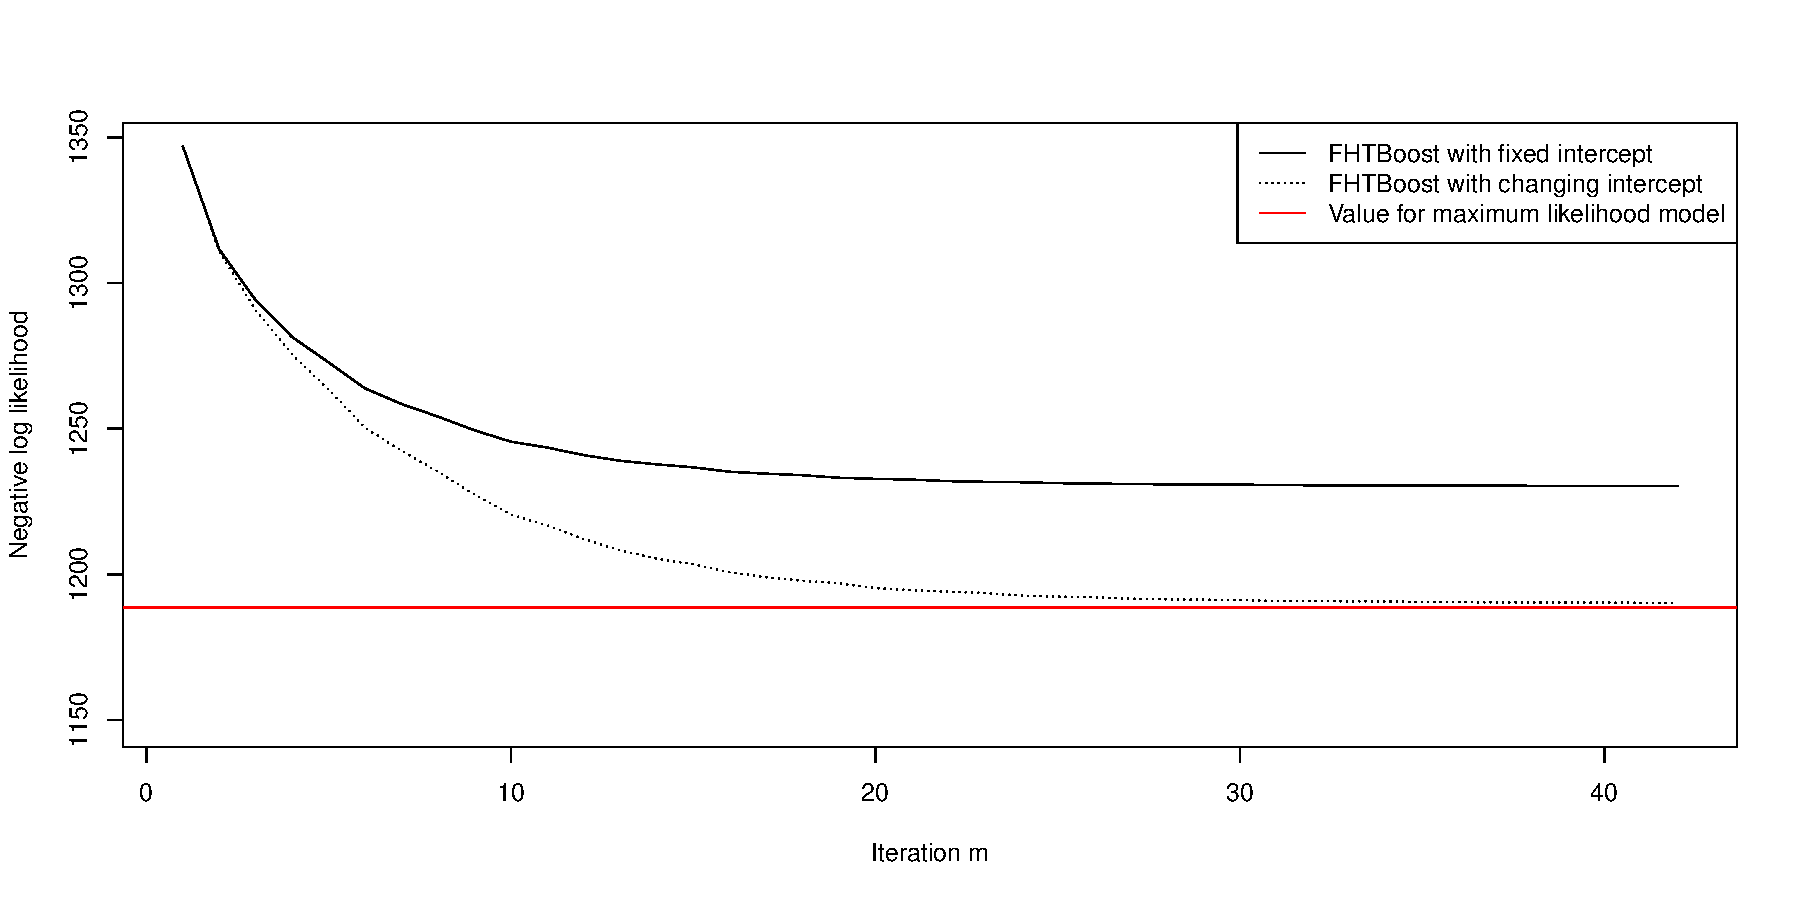
\includegraphics[scale=0.4]{figures/small_example.pdf}
\end{figure}
Figure \ref{fig:boosting-ML} shows a plot of the negative log likelihood of the data (in-sample loss) as a function of the iteration number $m$.
The solid black line shows negative log-likelihood for FHTBoost with a fixed intercept, i.e., the algorithm in the previous subsection.
With a fixed intercept, we only estimate the intercepts $\hat{\beta}_{0},\,\hat{\gamma}_{0}$ before we begin iterating, and so these intercepts are not changed in any of the boosting iterations.
The red line shows the negative of the maximum likelihood, obtained through numerical maximization of the joint maximum likelihood.
We can see in the figure \ref{fig:boosting-ML} that it quite clearly does not reach the maximum likelihood value, which is the solid red horizontal line.
The maximum likelihood intercepts are $\hat{\beta}^{\text{ML}}_{1,0}=1.98$ and $\hat{\beta}^{\text{ML}}_{2,0}=-1.02$, while running the boosting algorithm for $\mstop=42$ iterations produces estimates of the intercepts as $\hat{\beta}^{[\mstop]}_{0}=1.68$ and $\hat{\gamma}^{[\mstop]}_{0}=-0.71$, respectively.

We therefore see that to achieve the maximum likelihood, we have to modify the algorithm to incorporate updates in the intercepts while boosting.
To change the intercept in each boosting iteration, we can perform a new numerical maximization after each boosting step.
This means to perform the same kind of numerical maximization as is done initially, at the beginning of each iteration, using now the estimated additive predictors as offsets.
We denote the initially estimated intercept $\hat{\beta}_{1,0}$ as $\hat{\beta}_{1,0}^{[0]}$.
The intercepts in the additive predictors now become sums of boosted intercepts,
\begin{equation}
    \hat{\beta}_{0}=\hat{\beta}_{0}^{[0]}+\sum_{m=1}^{\mstop}\hat{\beta}_{0}^{[m]},
\end{equation}
and
\begin{equation}
    \hat{\gamma}_{0}=\hat{\gamma}_{0}^{[0]}+\sum_{m=1}^{\mstop}\hat{\gamma}_{0}^{[m]}.
\end{equation}
Here each $\hat{\beta}_{0}^{[m]}$ and $\hat{\gamma}_{0}^{[m]}$ are calculated in the intercept estimated in step $m$ of the boosting algorithm.

When introducing \textit{changing} intercepts, the algorithm was successful in recovering the maximum likelihood value and parameters.
See table \ref{table:ML} for the estimated parameter values, and graphically, in figure \ref{fig:boosting-ML}, where the convergence is plotted as a function of the number of boosting iterations.
\begin{table}\caption{Parameter values of a model which reaches ML}\label{table:ML}
\centering
\begin{tabular}{lcccccc}
\toprule
    & $\beta_{0}$ & $\beta_{1}$ & $\beta_{2}$ & $\gamma_{0}$ & $\gamma_{1}$ & $\gamma_{2}$ \\
\hline
Maximum likelihood estimate     &    1.98 &    0.10 &    0.21 &    -1.03 &    -0.09 &     0.12 \\
FHTBoost with fixed intercept                 &    1.68 &    0.10 &    0.18 &    -0.72 &    -0.06 &     0.09 \\
FHTBoost with changing intercept              &    1.97 &    0.10 &    0.18 &    -1.02 &    -0.09 &     0.12 \\
\bottomrule
\end{tabular}
\end{table}

In mboost, they seem to change the offset while boosting.
This must surely be a problem others have encountered while deriving boosting algorithms.

%The resulting survival times have the Kaplan-Meier plot shown in Figure \ref{fig:small-example-kaplan-meier}.
%\begin{figure}
%\caption{Kaplan-Meier plot of generated survival data from subsection \ref{subsec:algo-example}.}
%\label{fig:small-example-kaplan-meier}
%\centering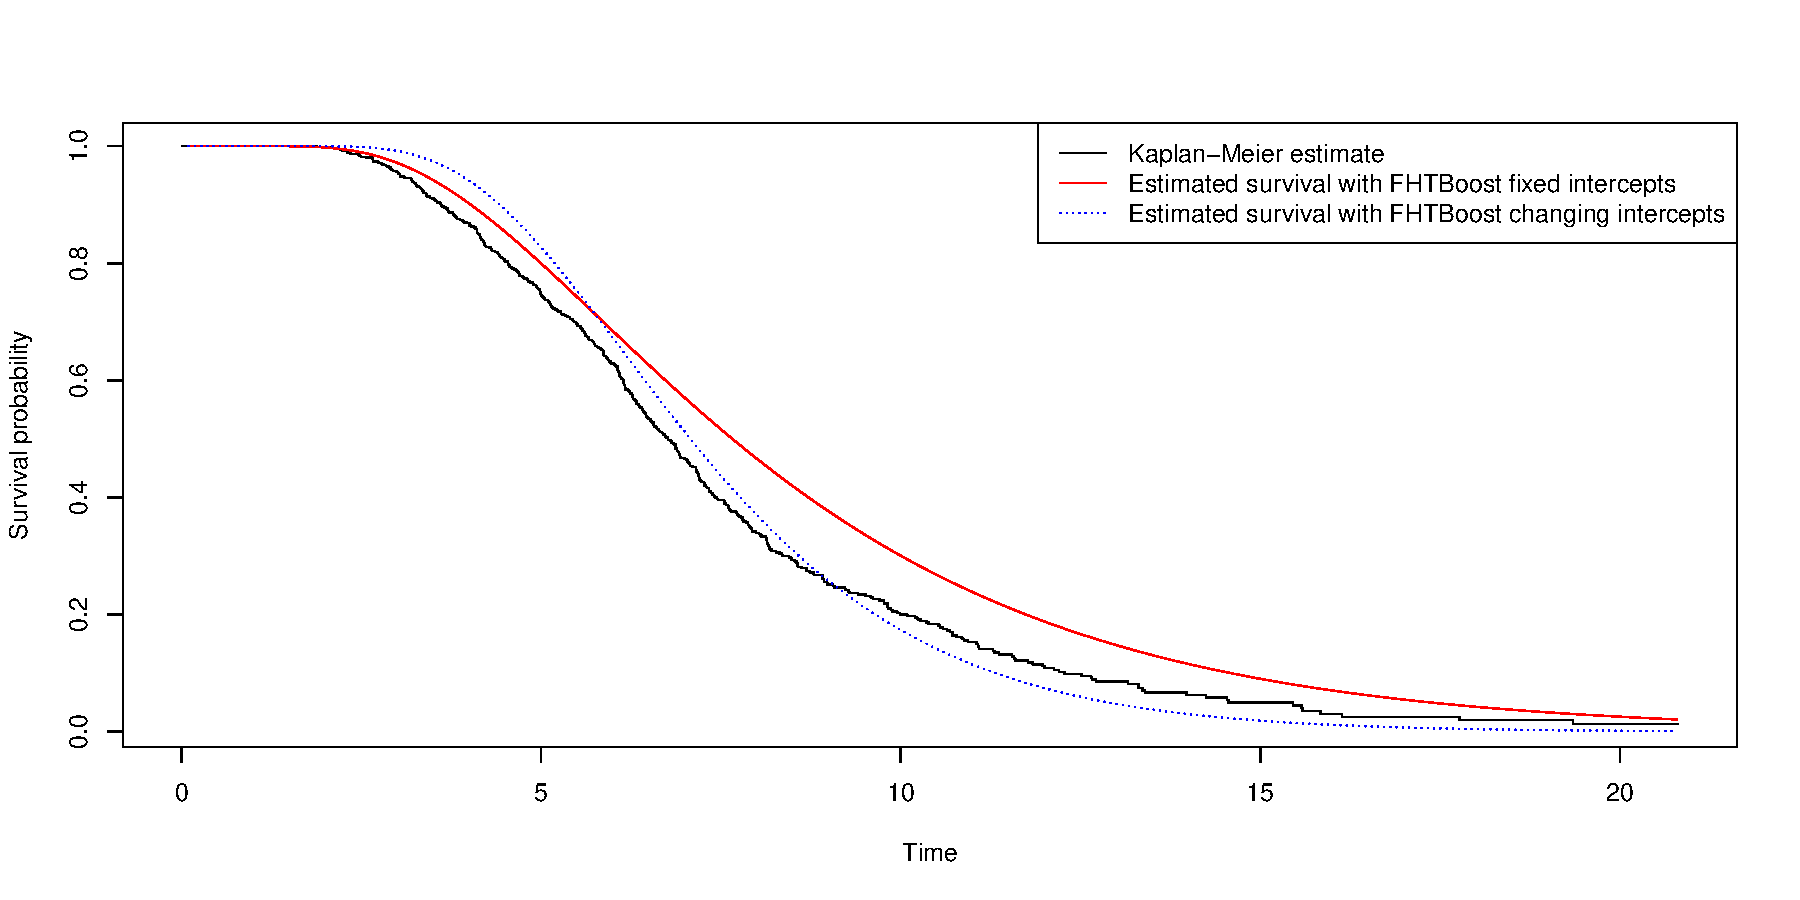
\includegraphics[scale=0.4]{figures/kaplan_meier_small.pdf}
%\end{figure}

\section{FHTBoost algorithm with changing intercept}\label{subsec:FHT-intercept}
%\begin{algorithm}
We modify algorithm \ref{algo:fhtboost}, where step \ref{algostep:FHT-end} is replaced by this step, where we incorporate changing intercepts for the additive predictors in each boosting iteration.
\label{algo:fhtboost-with-intercept}
\begin{enumerate}
    \setcounter{enumi}{12}
    \item
        Find which parameter should be included in the model,
        \begin{equation*}
            k^{[m]}=\argmin_{k\in\{1,2\}}\Delta\rho_k.
        \end{equation*}
        Include this component in the final model, by updating its additive predictor,
        \begin{equation*}
            \hat{\eta}^{[m]}_{k^{[m]}}=\hat{\eta}^{[m-1]}_{k^{[m]}}+\nu\cdot\hat{h}^{[m]}_{k^{[m]},\,j^{[m]}}(x),
        \end{equation*}
        while for the other component $k\neq k^{[m]}$, set the additive predictor for this iteration to be the same as previous iteration
        \begin{equation*}
            \hat{\eta}^{[m]}_{k}=\hat{\eta}^{[m-1]}_{k}.
        \end{equation*}
        Find the best numerical constant to add to the intercept of the selected additive learner,
        \begin{equation}
            c=\argmin_c \err\left(\hat{\boldeta}^{[m]}+c\right)
        \end{equation}
        Add this $c$ to the selected parameter
        \begin{equation}
            \hat{\beta}_{k^{[m]},0}\gets\hat{\beta}_{k^{[m]},0}+c.
        \end{equation}
\end{enumerate}
%\end{algorithm}

\section{Conclusion thoughts choices}
\todo[inline]{Write a conclusion from the example: The algorithm with updating intercept seems better, as it should not be shrunk towards 0 \citep{ESL}.}